\section{Wargame Scenario}
\label{sec:wargame}

The game can have up to four players, where some can be set to move in predefined patterns, so that one can get a feeling of playing against an artificial intelligence.\\
	When the wargame is initialized, the user chooses the size of the battle area, and the agents and teams are set up by the input of the generated XML-file \ref{agents_patterns}.\\
	The user can type his commands in the \textit{command center}, and execute them by pressing the \textit{Execute} button. When the user is done executing commands, he can end his turn by pressing \textit{End Turn}.\\
	The moves available for the user to make is up, down, left and right (one coordinate at a time), and it is also possible to make several moves with an agent, if you select the agent and type the coordinates you want the agent to move to.\\
  When a collision between agents from opposing teams occur, a random function is called, which decides which agent wins the fight, favoring the unit with the highest rank.
	
\begin{figure}[H]
\begin{center}
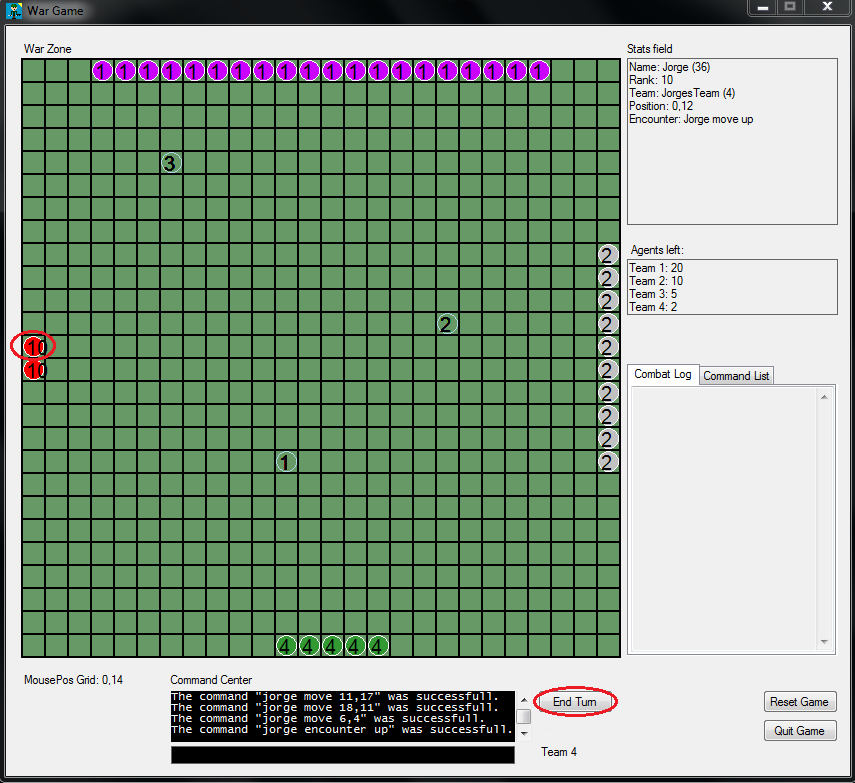
\includegraphics[scale=0.6]{Images/ex_com.png}
\end{center}
\caption{Example of an execution of a MOVE command. The user type the command \texttt{pink1 MOVE RIGHT 3} and press \textit{Execute}}
\label{fig:ex_com}
\end{figure}

\subsection{Agents and Action Patterns}
\label{agents_patterns}

%Something about how the agents, teams, squads and action patterns are set up...